\part{Counting}
\section{Handout 03: Binomial Theorem, Generalized Permutations and Combinations}

\subsection{Overview}

This handout completes Part~I on counting by introducing three major ideas:
\begin{itemize}[leftmargin=*]
    \item the \emph{binomial theorem} and basic binomial identities;
    \item the \emph{division rule}, which is the standard way to remove systematic overcounting;
    \item generalized counting models involving
    \begin{itemize}[leftmargin=*]
        \item cyclic arrangements,
        \item repetition,
        \item indistinguishable objects,
        \item distributions into boxes.
    \end{itemize}
\end{itemize}

The main exam skill in this handout is to distinguish among the following situations:
\[
\begin{aligned}
&\text{ordered vs unordered}, &&
\text{with repetition vs without repetition},\\
&\text{distinguishable vs indistinguishable}, &&
\text{linear vs cyclic}.
\end{aligned}
\]

\begin{examtip}[title={Main modelling checklist for Handout 03}]
Before writing any formula, decide all four of the following:
\begin{enumerate}[leftmargin=*]
    \item Does order matter?
    \item Is repetition allowed?
    \item Are equal-looking objects actually indistinguishable?
    \item Are two arrangements identified by rotation?
\end{enumerate}
Most errors in this handout come from answering one of these four questions incorrectly.
\end{examtip}

%==================================================
\subsection{The Binomial Theorem}
%==================================================

\begin{theorem}{Binomial Theorem}{binomial-theorem}
Let $x$ and $y$ be variables and let $n$ be a nonnegative integer. Then
\[
(x+y)^n
=
\sum_{i=0}^{n}\binom{n}{i}x^{\,n-i}y^i.
\]
Equivalently,
\[
(x+y)^n
=
\binom{n}{0}x^n+\binom{n}{1}x^{n-1}y+\cdots+\binom{n}{n-1}xy^{n-1}+\binom{n}{n}y^n.
\]
\end{theorem}

\begin{proof}
Expand
\[
(x+y)^n=(x+y)(x+y)\cdots(x+y)
\]
as a product of $n$ identical factors. A term of the form
\[
x^{n-i}y^i
\]
arises precisely when one chooses $y$ from exactly $i$ of the $n$ factors, and therefore $x$ from the remaining $n-i$ factors. The number of such choices is
\[
\binom{n}{i}.
\]
Hence the coefficient of $x^{n-i}y^i$ is $\binom{n}{i}$, giving the formula.
\end{proof}

\begin{keyformula}[title={Binomial theorem}]
\[
(x+y)^n=\sum_{i=0}^{n}\binom{n}{i}x^{\,n-i}y^i.
\]
\end{keyformula}

\subsubsection{Coefficient extraction}

A binomial expansion question is often a coefficient question. One identifies the exponent pattern first, then determines which index $i$ is required.

\begin{examplebox}[title={Expansion of $(x+y)^4$}]
By the binomial theorem,
\[
(x+y)^4
=
\sum_{i=0}^{4}\binom{4}{i}x^{4-i}y^i
=
x^4+4x^3y+6x^2y^2+4xy^3+y^4.
\]
\end{examplebox}

\begin{examplebox}[title={Coefficient of $x^{12}y^{13}$ in $(x+y)^{25}$}]
In the general term
\[
\binom{25}{i}x^{25-i}y^i,
\]
we require
\[
25-i=12,\qquad i=13.
\]
Hence the coefficient is
\[
\binom{25}{13}=\frac{25!}{13!12!}=5{,}200{,}300.
\]
\end{examplebox}

\begin{examplebox}[title={Coefficient of $x^{12}y^{13}$ in $(2x-3y)^{25}$}]
Using the binomial theorem with $2x$ in place of $x$ and $-3y$ in place of $y$,
\[
(2x-3y)^{25}
=
\sum_{i=0}^{25}\binom{25}{i}(2x)^{25-i}(-3y)^i.
\]
To obtain $x^{12}y^{13}$, we again take $i=13$. Therefore the coefficient is
\[
\binom{25}{13}2^{12}(-3)^{13}.
\]
\end{examplebox}

\begin{commonmistake}[title={Coefficient questions with scaled variables}]
In expressions such as $(2x-3y)^n$, the coefficient is \emph{not} just a binomial coefficient. One must also include the powers of the numerical multipliers and the sign.
\end{commonmistake}

\begin{extension}[title={Why the coefficient is a combination}]
The coefficient of $x^{n-i}y^i$ counts the number of ways to choose exactly which $i$ factors contribute the $y$ term. This is why binomial coefficients appear naturally: every monomial in the expansion corresponds to a subset of the $n$ factor positions.
\end{extension}

%==================================================
\subsection{Basic Binomial Identities}
%==================================================

\begin{theorem}{Sum of the binomial coefficients}{sum-binomial}
For every nonnegative integer $n$,
\[
\sum_{i=0}^{n}\binom{n}{i}=2^n.
\]
\end{theorem}

\begin{proof}
Substitute $x=1$ and $y=1$ into the binomial theorem:
\[
2^n=(1+1)^n=\sum_{i=0}^{n}\binom{n}{i}1^{n-i}1^i=\sum_{i=0}^{n}\binom{n}{i}.
\]
\end{proof}

\begin{examplebox}[title={Combinatorial meaning of $\sum_{i=0}^{n}\binom{n}{i}=2^n$}]
Let $S$ be an $n$-element set. The quantity $2^n$ counts all subsets of $S$. On the other hand, for each $i$ there are $\binom{n}{i}$ subsets of size $i$. Summing over all possible sizes gives
\[
\sum_{i=0}^{n}\binom{n}{i}=2^n.
\]
\end{examplebox}

\begin{theorem}{Pascal's Identity}{pascal-identity}
For integers $n\ge r\ge 1$,
\[
\binom{n+1}{r}=\binom{n}{r}+\binom{n}{r-1}.
\]
\end{theorem}

\begin{proof}
Count the $r$-element subsets of an $(n+1)$-element set $S$. Fix one distinguished element $a\in S$, and let $T=S\setminus\{a\}$, so $|T|=n$.

Every $r$-element subset of $S$ falls into exactly one of two disjoint classes:
\begin{itemize}[leftmargin=*]
    \item those that do not contain $a$, of which there are $\binom{n}{r}$;
    \item those that contain $a$, in which case the remaining $r-1$ elements must be chosen from $T$, giving $\binom{n}{r-1}$.
\end{itemize}
Adding the two disjoint classes gives
\[
\binom{n+1}{r}=\binom{n}{r}+\binom{n}{r-1}.
\]
\end{proof}

% Pascal triangle fragment illustrating Pascal's identity row-by-row
\begin{center}
\begin{tikzpicture}[x=1cm,y=0.65cm]
\node at (0,0) {$1$};
\node at (-0.5,-1) {$1$}; \node at (0.5,-1) {$1$};
\node at (-1,-2) {$1$}; \node at (0,-2) {$2$}; \node at (1,-2) {$1$};
\node at (-1.5,-3) {$1$}; \node at (-0.5,-3) {$3$}; \node at (0.5,-3) {$3$}; \node at (1.5,-3) {$1$};
\node at (-2,-4) {$1$}; \node at (-1,-4) {$4$}; \node at (0,-4) {$6$}; \node at (1,-4) {$4$}; \node at (2,-4) {$1$};
\draw[->,gray] (-1,-2.4) -- (-0.15,-3.6);
\draw[->,gray] (0,-2.4) -- (-0.15,-3.6);
\end{tikzpicture}
\end{center}

\begin{extension}[title={Structural meaning of Pascal's identity}]
Pascal's identity is a prototype of a counting argument by partition. The right-hand side arises by splitting a family of subsets into two disjoint classes according to whether a distinguished element is present.
\end{extension}

%==================================================
\subsection{Division Rule}
%==================================================

The division rule is the standard tool for correcting uniform overcounting.

\begin{definition}{A $k$-to-$1$ function}{k-to-1}
A function $f:X\to Y$ is called \emph{$k$-to-$1$} if for every $y\in Y$, there are exactly $k$ elements $x\in X$ such that
\[
f(x)=y.
\]
\end{definition}

\begin{theorem}{Division Rule}{division-rule}
If $f:X\to Y$ is a $k$-to-$1$ function between finite sets, then
\[
|Y|=\frac{|X|}{k}.
\]
\end{theorem}

\begin{proof}
Because every element of $Y$ has exactly $k$ preimages, the set $X$ is partitioned into $|Y|$ disjoint fibres, each of size $k$. Hence
\[
|X|=k|Y|,
\]
and therefore
\[
|Y|=\frac{|X|}{k}.
\]
\end{proof}

\begin{keyformula}[title={Division rule}]
\[
\text{If a known set }X\text{ maps }k\text{-to-}1\text{ onto }Y,\text{ then }|Y|=\frac{|X|}{k}.
\]
\end{keyformula}

\begin{examtip}[title={When the division rule appears}]
Use the division rule whenever several linear descriptions represent the same final object. The main task is then to determine the overcounting factor $k$ exactly.
\end{examtip}

%==================================================
\subsection{Permutations Around a Cycle}
%==================================================

A cyclic arrangement identifies linear orders that differ only by rotation.

\begin{theorem}{Cyclic $r$-permutations}{cycle-permutation}
The number of ways to choose $r$ elements from an $n$-element set and arrange them around a cycle is
\[
\frac{1}{r}P(n,r)=\frac{n!}{r(n-r)!}.
\]
\end{theorem}

\begin{proof}
Let $P$ be the set of all linear $r$-permutations of the given $n$-element set, so
\[
|P|=P(n,r).
\]
Let $C$ be the set of cyclic arrangements of $r$ distinct chosen elements.

Define a map
\[
f:P\to C
\]
by sending a linear arrangement $(a_1,a_2,\dots,a_r)$ to the corresponding cyclic arrangement with the same circular order.

For a fixed cyclic arrangement, there are exactly $r$ linear arrangements mapping to it, namely the $r$ cyclic shifts
\[
(a_1,a_2,\dots,a_r),\ (a_2,a_3,\dots,a_r,a_1),\ \dots,\ (a_r,a_1,\dots,a_{r-1}).
\]
Hence $f$ is $r$-to-$1$. By the division rule,
\[
|C|=\frac{|P|}{r}=\frac{P(n,r)}{r}=\frac{n!}{r(n-r)!}.
\]
\end{proof}

% Cyclic arrangement equivalence under rotation
\begin{center}
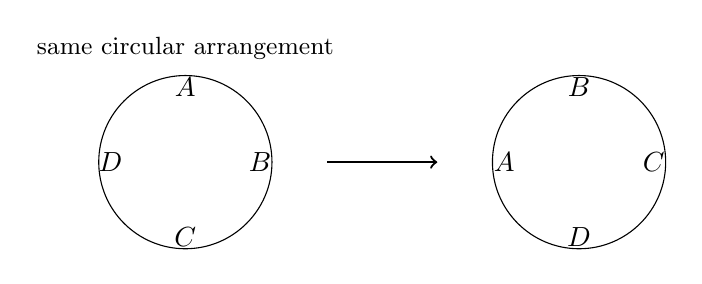
\begin{tikzpicture}[scale=1]
\draw (0,0) circle (1.1);
\node at (0,1.45) {\small same circular arrangement};
\node at (0,0.95) {$A$};
\node at (0.95,0) {$B$};
\node at (0,-0.95) {$C$};
\node at (-0.95,0) {$D$};

\draw[->,thick] (1.8,0) -- (3.2,0);

\draw (5,0) circle (1.1);
\node at (5,0.95) {$B$};
\node at (5.95,0) {$C$};
\node at (5,-0.95) {$D$};
\node at (4.05,0) {$A$};
\end{tikzpicture}
\end{center}

\begin{examplebox}[title={Three students around a table}]
The number of ways to seat $3$ students around a round table is
\[
\frac{P(3,3)}{3}=\frac{3!}{3}=2.
\]
Thus there are exactly two cyclic arrangements.
\end{examplebox}

\begin{examplebox}[title={Choosing and seating $r$ students around a round table}]
If one must choose $r$ students from $n$ and then seat them around a round table, the answer is
\[
\frac{1}{r}P(n,r)=\frac{n!}{r(n-r)!}.
\]
This is the direct application of the theorem above.
\end{examplebox}

\begin{commonmistake}[title={Linear order versus cyclic order}]
For a linear arrangement, different starting positions matter; for a cyclic arrangement, they do not. Dividing by $r$ is valid only because all $r$ chosen elements are distinct and every cyclic arrangement has exactly $r$ linear representatives.
\end{commonmistake}

\begin{extension}[title={Division by symmetry}]
The factor $r$ arises from rotational symmetry. More generally, whenever a symmetry group acts freely on a set of linear descriptions, the number of genuinely different configurations is obtained by dividing by the orbit size.
\end{extension}

%==================================================
\subsection{Permutations With Repetition}
%==================================================

\begin{theorem}{$r$-permutations with repetition}{perm-with-repetition}
The number of ordered strings of length $r$ formed from a set of $n$ elements, when repetition is allowed, is
\[
n^r.
\]
\end{theorem}

\begin{proof}
Each of the $r$ positions may be filled independently with any of the $n$ available elements. By the product rule, the total number of strings is
\[
\underbrace{n\cdot n\cdots n}_{r\text{ times}}=n^r.
\]
\end{proof}

\begin{keyformula}[title={Ordered selection with repetition}]
\[
\text{number of length-}r\text{ strings from }n\text{ symbols}=n^r.
\]
\end{keyformula}

\begin{examplebox}[title={Strings over the English alphabet}]
The number of strings of length $r$ formed from the English alphabet is
\[
26^r,
\]
since each of the $r$ positions has $26$ choices.
\end{examplebox}

\begin{examplebox}[title={Four-digit PIN code}]
If digits may repeat, then a four-digit PIN code has
\[
10^4=10{,}000
\]
possible ordered strings.
\end{examplebox}

%==================================================
\subsection{Combinations With Repetition}
%==================================================

Here order does not matter, but repetition is allowed.

\begin{theorem}{$r$-combinations with repetition}{comb-with-repetition}
The number of $r$-combinations from a set with $n$ elements, when repetition is allowed, is
\[
\binom{n+r-1}{r}=\binom{n+r-1}{n-1}.
\]
\end{theorem}

\begin{proof}
Interpret an $r$-combination with repetition as distributing $r$ indistinguishable balls into $n$ distinguishable bins, where the $i$-th bin records how many copies of the $i$-th element are chosen.

Represent such a distribution by a string consisting of
\[
r\text{ balls }(\bullet)\quad\text{and}\quad n-1\text{ dividers }(|).
\]
For example, the string
\[
\bullet\bullet\,|\,|\,\bullet\,|\,\bullet
\]
with $n=4$ and $r=4$ corresponds to the multiset containing $2$ copies of the first element, $0$ copies of the second, $1$ copy of the third, and $1$ copy of the fourth.

Thus every $r$-combination with repetition corresponds bijectively to a string of length
\[
r+(n-1)=n+r-1
\]
containing $r$ balls and $n-1$ dividers. Such a string is determined by choosing the positions of the $r$ balls (or, equivalently, the $n-1$ dividers). Hence the number of such strings is
\[
\binom{n+r-1}{r}=\binom{n+r-1}{n-1}.
\]
\end{proof}

\begin{keyformula}[title={Unordered selection with repetition}]
\[
\text{number of }r\text{-combinations from }n\text{ elements with repetition}
=
\binom{n+r-1}{r}.
\]
\end{keyformula}

% Stars and bars representation for a multiset selection
\begin{center}
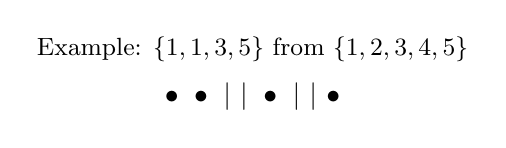
\begin{tikzpicture}[x=0.5cm,y=0.5cm]
\node at (0,1.2) {\small Example: $\{1,1,3,5\}$ from $\{1,2,3,4,5\}$};
\node at (0,0) {$\bullet\ \bullet\ |\ |\ \bullet\ |\ |\ \bullet$};
\end{tikzpicture}
\end{center}

\begin{examplebox}[title={Selecting fruit}]
How many ways are there to select $3$ pieces of fruit from a bowl containing apples, oranges, and pears, if order does not matter?

\textbf{Solution.}
This is a $3$-combination from a set of $3$ fruit types with repetition allowed. Hence the answer is
\[
\binom{3+3-1}{3}=\binom{5}{3}=10.
\]
\end{examplebox}

\begin{examplebox}[title={Cookie shop}]
A cookie shop offers $4$ kinds of cookies. The number of ways to choose $6$ cookies, if order does not matter, is
\[
\binom{4+6-1}{6}=\binom{9}{6}=84.
\]
\end{examplebox}

\subsubsection{Nonnegative integer solutions}

The stars-and-bars theorem is equivalent to counting nonnegative integer solutions.

\begin{theorem}{Nonnegative solutions of a linear equation}{nonnegative-solutions}
The number of solutions in nonnegative integers to
\[
x_1+x_2+\cdots+x_n=r
\]
is
\[
\binom{n+r-1}{r}.
\]
\end{theorem}

\begin{proof}
A solution $(x_1,\dots,x_n)$ specifies how many of the $r$ indistinguishable objects are placed into each of the $n$ labelled bins. This is precisely the same model as $r$-combinations with repetition from an $n$-element set, so the answer is
\[
\binom{n+r-1}{r}.
\]
\end{proof}

\begin{examplebox}[title={Equation $x_1+x_2+x_3=11$}]
The number of nonnegative integer solutions of
\[
x_1+x_2+x_3=11
\]
is
\[
\binom{3+11-1}{11}=\binom{13}{11}=\binom{13}{2}=78.
\]
\end{examplebox}

\begin{examplebox}[title={Lower bounds by shifting variables}]
How many integer solutions are there to
\[
x_1+x_2+x_3=11,
\qquad
x_1\ge 1,\ x_2\ge 2,\ x_3\ge 3?
\]

\textbf{Solution.}
Write
\[
x_1=1+y_1,\qquad x_2=2+y_2,\qquad x_3=3+y_3,
\]
where $y_1,y_2,y_3\ge 0$. Then
\[
y_1+y_2+y_3=11-(1+2+3)=5.
\]
Hence the number of solutions is
\[
\binom{3+5-1}{5}=\binom{7}{5}=\binom{7}{2}=21.
\]
\end{examplebox}

\begin{extension}[title={Canonical stars-and-bars encoding}]
The stars-and-bars argument is a canonical bijection: a multiset choice is fully determined by the multiplicity of each symbol, and these multiplicities are encoded by block lengths between dividers. This is why the same formula also counts nonnegative integer solutions.
\end{extension}

\begin{commonmistake}[title={Repetition allowed does not mean order matters}]
The formulas
\[
n^r
\qquad\text{and}\qquad
\binom{n+r-1}{r}
\]
both involve repetition, but they count different objects. The first counts ordered strings; the second counts unordered selections.
\end{commonmistake}

%==================================================
\subsection{Permutations With Indistinguishable Objects}
%==================================================

\begin{theorem}{Permutations of indistinguishable objects}{indistinguishable-perm}
Suppose there are $n$ objects in total, with
\[
n_1\text{ objects of type }1,\quad
n_2\text{ objects of type }2,\quad
\dots,\quad
n_k\text{ objects of type }k,
\]
where
\[
n_1+n_2+\cdots+n_k=n.
\]
Then the number of distinct permutations is
\[
\frac{n!}{n_1!n_2!\cdots n_k!}.
\]
\end{theorem}

\begin{proof}
First pretend that all objects are distinguishable. Then there are $n!$ linear permutations.

Now pass to the setting in which objects of the same type are indistinguishable. Different labelings of the identical objects produce the same final arrangement. For each final arrangement, the objects of type $1$ can be internally relabelled in $n_1!$ ways, those of type $2$ in $n_2!$ ways, and so on. Hence every distinct arrangement is represented exactly
\[
n_1!n_2!\cdots n_k!
\]
times among the $n!$ labelled permutations.

By the division rule, the number of distinct permutations is
\[
\frac{n!}{n_1!n_2!\cdots n_k!}.
\]
\end{proof}

\begin{keyformula}[title={Indistinguishable objects}]
\[
\text{number of distinct permutations}
=
\frac{n!}{n_1!n_2!\cdots n_k!}.
\]
\end{keyformula}

\begin{examplebox}[title={The word SUCCESS}]
The word \texttt{SUCCESS} has $7$ letters with multiplicities
\[
S^3,\quad C^2,\quad U^1,\quad E^1.
\]
Hence the number of distinct rearrangements is
\[
\frac{7!}{3!2!1!1!}=420.
\]
\end{examplebox}

\begin{examplebox}[title={The word MISSISSIPPI}]
The word \texttt{MISSISSIPPI} has $11$ letters with multiplicities
\[
I^4,\quad S^4,\quad P^2,\quad M^1.
\]
Therefore the number of distinct rearrangements is
\[
\frac{11!}{4!4!2!1!}=34{,}650.
\]
\end{examplebox}

\begin{extension}[title={Label-then-divide strategy}]
A reliable way to count with indistinguishable objects is:
\begin{enumerate}[leftmargin=*]
    \item temporarily label identical objects so that everything becomes distinguishable;
    \item count the labelled arrangements;
    \item divide by the number of relabellings that do not change the final visible arrangement.
\end{enumerate}
This is one of the most useful recurring patterns in advanced counting.
\end{extension}

%==================================================
\subsection{Distributions Into Boxes}
%==================================================

\subsubsection{Distinguishable objects into distinguishable boxes}

\begin{theorem}{Specified occupancy distribution}{box-distribution}
The number of ways to distribute $n$ distinguishable objects into $k$ distinguishable boxes so that box $1$ receives $n_1$ objects, box $2$ receives $n_2$ objects, \dots, box $k$ receives $n_k$ objects, where
\[
n_1+n_2+\cdots+n_k=n,
\]
is
\[
\frac{n!}{n_1!n_2!\cdots n_k!}.
\]
\end{theorem}

\begin{proof}
Choose which $n_1$ objects go to box $1$, then which $n_2$ of the remaining objects go to box $2$, and so on. The count is
\[
\binom{n}{n_1}\binom{n-n_1}{n_2}\cdots \binom{n-n_1-\cdots-n_{k-1}}{n_k}.
\]
Simplifying this product yields
\[
\frac{n!}{n_1!n_2!\cdots n_k!}.
\]
\end{proof}

\begin{examplebox}[title={Distribution with fixed box sizes}]
The number of ways to distribute $8$ distinct objects into $3$ distinct boxes so that the box sizes are $3,2,3$ is
\[
\frac{8!}{3!2!3!}=560.
\]
\end{examplebox}

\subsubsection{Indistinguishable objects into distinguishable boxes}

If the objects are indistinguishable and the boxes are distinguishable, one is counting nonnegative integer solutions.

\begin{examplebox}[title={Five indistinguishable objects into three distinguishable boxes}]
The number of ways to distribute $5$ indistinguishable objects into $3$ distinguishable boxes is the number of nonnegative integer solutions of
\[
x_1+x_2+x_3=5.
\]
Hence the answer is
\[
\binom{3+5-1}{5}=\binom{7}{5}=\binom{7}{2}=21.
\]
\end{examplebox}

\subsubsection{Optional viewpoints from the handout}

\begin{extension}[title={Distinguishable objects into indistinguishable boxes}]
When the boxes are indistinguishable, there is generally no similarly simple closed formula. The handout treats this by breaking into cases and, optionally, via Stirling numbers of the second kind:
\[
S(n,j)=\frac{1}{j!}\sum_{i=0}^{j-1}(-1)^i\binom{j}{i}(j-i)^n.
\]
These count the ways to distribute $n$ distinguishable objects into $j$ indistinguishable nonempty boxes.
\end{extension}

\begin{extension}[title={Indistinguishable objects into indistinguishable boxes}]
This becomes a partition problem. The number of ways to distribute $n$ indistinguishable objects into at most $k$ indistinguishable boxes is the number of partitions of $n$ into at most $k$ positive parts, often denoted by $p_k(n)$.
\end{extension}

%==================================================
\subsection{Special Techniques}
%==================================================

\subsubsection*{1. Coefficient targeting in binomial expansions}
When asked for a specific coefficient, match exponents first. Only after identifying the correct index should you substitute the associated binomial coefficient and numerical multipliers.

\subsubsection*{2. Count first, then divide}
If many linear descriptions represent the same final object, count the linear descriptions and divide by the uniform overcounting factor. This is the main mechanism behind cyclic permutations and indistinguishable objects.

\subsubsection*{3. Stars and bars}
Whenever the problem is about unordered selection with repetition, or nonnegative integer solutions to a sum equation, try to convert the problem into placing balls and dividers in a line.

\subsubsection*{4. Shift lower bounds away}
For constraints such as
\[
x_i\ge a_i,
\]
write
\[
x_i=a_i+y_i,\qquad y_i\ge 0,
\]
and reduce the problem to a standard nonnegative-solution count.

\subsubsection*{5. Label identical objects temporarily}
For problems involving repeated letters or identical objects, first pretend the copies are distinct, count all permutations, then divide by the internal relabellings.

\subsubsection*{6. Diagnose the symmetry}
If a problem involves round tables, necklaces, rotations, repeated letters, or any other visible identification of multiple linear arrangements, ask immediately whether the same visible arrangement is being counted several times.

\begin{examtip}[title={High-yield distinction table}]
A quick diagnostic:
\[
\begin{array}{c|c}
\text{Situation} & \text{Typical formula} \\ \hline
\text{ordered, no repetition} & P(n,r)=\dfrac{n!}{(n-r)!} \\
\text{ordered, repetition allowed} & n^r \\
\text{unordered, no repetition} & \binom{n}{r} \\
\text{unordered, repetition allowed} & \binom{n+r-1}{r} \\
\text{indistinguishable copies in a line} & \dfrac{n!}{n_1!\cdots n_k!} \\
\text{around a cycle} & \dfrac{P(n,r)}{r}
\end{array}
\]
Always verify that the modelling assumptions match the row you use.
\end{examtip}

%==================================================
\subsection{Summary Table}
%==================================================

\begin{center}
\scriptsize
\begin{tabular}{@{}p{0.28\textwidth}p{0.27\textwidth}p{0.27\textwidth}@{}}
\toprule
& \textbf{$r$-permutation} & \textbf{$r$-combination} \\
\midrule
without repetition
&
\[
P(n,r)=\frac{n!}{(n-r)!}
\]
&
\[
\binom{n}{r}=\frac{n!}{(n-r)!r!}
\]
\\[1.0em]
with repetition
&
\[
n^r
\]
&
\[
\binom{n+r-1}{r}
\]
\\[1.0em]
with indistinguishable objects
&
\[
\frac{n!}{n_1!n_2!\cdots n_k!}
\]
&
\text{use multiplicities / multiset model}
\\[1.0em]
around a cycle
&
\[
\frac{P(n,r)}{r}
=
\frac{n!}{r(n-r)!}
\]
&
\text{not a standard separate formula}
\\
\bottomrule
\end{tabular}
\end{center}

\begin{commonmistake}[title={Final warning for Handout 03}]
The formulas in this handout are similar in appearance but answer different questions. Never choose a formula just because it looks familiar. First classify the problem by order, repetition, indistinguishability, and cyclic symmetry; only then substitute a formula.
\end{commonmistake}
